\chapter{Методы построения маршрутов}
Сформулируем постановку задачи формирования маршрутов. Пусть заданы \( N_s \) – число узлов (остановочных 
пунктов), \( N_r \) – число маршрутов. Требуется построить \( N_r \) последовательностей узлов, при которых 
целевая функция качества маршрутной сети будет принимать максимальное значение. 

Задача тесно связана с задачей маршрутизацией <<из пункта А в пункт Б>>, но имеет некоторые отличия. 
Во-первых, в типовой задаче маршрутизации целевая функция – это время поездки от начала до конца маршрута, 
которое необходимо минимизировать. В случае с построением сети маршрутов общественного транспорта целевая 
функция -- интегральная, учитывающая средние показатели времени пешего хода до остановки, длины пути, 
количества пересадок, и пр. \cite{bib:9,bib:17}. Во-вторых, в типовой задаче маршрутизации для движения 
выбираются любые промежуточные точки, сокращающие маршрут, тогда как в рассматриваемой задаче промежуточные 
точки расположены там же, где и центры кластеров.

Предлагается две стратегии генерации исходной сети маршрутов общественного транспорта. Первая предполагает 
генерацию одного <<длинного>> маршрута, обходящего все исходные узлы. Далее осуществляется разрез маршрута 
на \( N_r \) маршрутов и осуществляется модификация сети в соответствии с эволюционным алгоритмом. Вторая 
стратегия: формирование начальной сети, число маршрутов в которой соответствует заданному значению \( N_r \) 
и применение эволюционных алгоритмов для поиска сети маршрутов с минимальной длиной. Но для начала рассмотрим 
некоторые алгоритмы применимые к данной задаче, прежде чем перейдём к \ref{sec:second_alg} и 
\ref{sec:third-alg}.

\section{Проанализированные алгоритмы}
\subsection{Методы локального поиска}
\emph{Алгоритмы локального поиска} -- группа алгоритмов, в которых поиск ведется только на основании текущего 
состояния, а ранее пройденные состояния не учитываются и не запоминаются. Основной целью поиска является не 
нахождение оптимального пути к целевой точке, а оптимизация некоторой целевой функции, поэтому задачи, 
решаемые подобными алгоритмами, называют задачами оптимизации. Для описания пространства состояний в таких 
задачах используют ландшафт пространства состояний, в этом представлении задача сводится к поиску состояния 
глобального максимума (или минимума) на данном ландшафте.

Методы локального поиска можно представить следующий общим алгоритмом \ref{alg:local-search}.
\begin{algorithm}[ht!]
    \caption{Общий алгоритм локального поиска}
    \KwData{\( A \) -- начальное решение}
    \KwResult{\( S \) -- результат алгоритма}
    \( S \leftarrow \) начальное решение \( A \)\;
    \While{в окрестности есть \( R \): \( f(R) > f(S) \)}{
        Заменить \( S \) на \( R \)\;
    }
    \label{alg:local-search}
\end{algorithm}

\emph{Алгоритм последовательного улучшения:} классический вариант локального спуска с монотонным 
улучшением по целевой функции. \emph{Основная проблема:} вероятность <<свалиться>> в локальный оптимум.

\emph{Алгоритм порогового улучшения:} пороговая последовательность постепенно убывает до нуля. Вариант 
когда допускается ухудшение по целевой функции до некоторого заданного порога, и этот порог постепенно 
снижается до нуля. \emph{Основная проблема:} чувствительность данных к пороговому значению.

\subsection{Жадный рандомизированный адаптивный поиск}
\emph{Основная суть алгоритма}: создаёться допустимое решение путём его конструирования из компонент с 
максимальной стоимостью, а затем осуществляеться локальный поиск в окрестности найденого решения.

Псевдокод алгоритма:
\begin{enumerate}
    \item построение решение кандидата
    \begin{enumerate}
        \item оценка невключенных элементов в решение с помощью эврестической функции
        \item сохранение лучших элементов в списке кандидатов
    \end{enumerate}
    \item последующее улучшение решения с помощью локального поиска
\end{enumerate}

\emph{Основная проблема:} игнорирование локально неоптимальных решение сильно влиющих на конечный результат.

\subsection{Метод поиска чередующихся окрестностей}
Метод чередующихся окрестностей -- это метаэвристика локального поиска, которая использует окрестности для 
ухода от плохих локальных оптимумов. Основная идея данного метода состоит в последовательном изучении набора
предопределенных окрестностей для получения лучшего решения. Алгоритм использует метод спуска для получения 
локального минимума. Затем он исследует случайно либо систематически множество окрестностей. Текущее решение 
заменяется новым лучшим решение. Поиск начинается с первой окрестности. Если решение, лучшее, чем текущее, 
там не будет найдено, алгоритм переходит к следующей окрестности, случайным образом генерирует новое решение, 
и пытается улучшить его. Когда в данной окрестности найден локальный оптимум, выбирается другая окрестность, 
которая используется на следующих итерациях. Таким образом, для данного множества окрестностей решение 
порождается случайным образом в первой окрестности текущего решения, из которого выполняется локальный спуск.

Данный алгоритм основан на следующих замечаниях:
\begin{enumerate}
    \item локальный оптимум относительно одной окрестности может не быть им относительно другой 
        окрестности;
    \item глобальный оптимум являеться локальным оптимумом относительно любой окрестности/
\end{enumerate}

Краткие по замечания по алгоритму:
\begin{enumerate}
    \item использование окрестностей для ухода от неоптимальных локальных оптимумов;
    \item использование метода спуска для получения локального оптимума;
    \item изучение набора предопределенных окрестностей для получения лучшего решения;
    \item переход к новой окрестности и генерация случайного решения при отсутсвии лучшего решения.
\end{enumerate}

\emph{Основная проблема:} получение локально оптмального решения.

\subsection{Метод имитации отжига}
Эта метаэвристика является рандомизированным методом локального поиска, позволяющим избежать плохих локальных 
оптимумов. Имитация отжига исходит из аналогии с физическим процессом отжига, направленным на получение 
твердых тел с низкой энергией состояния. В физике конденсированного состояния отжиг является процессом, в 
котором твердое тело сначала расплавляют путем увеличения температуры, затем постепенно снижают температуру
для восстановления твердого состояния с низкой энергией. Метод имитации отжига -- это стохастический метод 
поиска, в котором на каждом шаге текущее решение заменяется другим, случайно выбранным из окрестности и 
улучшающим значение целевой функции решением. Метод использует управляющий параметр, именуемый температурой, 
для определения вероятности принятия решений, не улучшающих значение целевой функции. Температура постепенно 
снижается согласно графику охлаждения так, что отдельные не улучшающие значение целевой функции решения 
принимаются в конце поиска.

В отличие от большинства метаэвристик, для алгоритма имитации отжига доказана асимптотическая сходимость к 
глобальному оптимуму. 

Основные положения по методу
\begin{itemize}
    \item этап принятия решения отличный от локального поиска
    \[
        P(T, R, S)= \left\{\begin{array}{cc}
            1                       & \text{если } S \leq R, \\
            \exp\frac{f(S)-f(R)}{T} & \text{если } S > R,
        \end{array}\right.
    \]
    \item необходим подбор начальных значений
    \item введение ограничений по времени / количеству итераций
\end{itemize}

Здесь \( T \) -- темпертура процесса, \( f \) -- целевая функция, \( S \) -- исходное решение, 
\( R \) -- решение кандидат.

Псевдокод алгоритма можно представить в следующем виде \ref{alg:simulated-anealing}.

\newpage

\begin{algorithm}[ht!]
    \caption{Общий алгоритм имитации отжига}
    \KwData{\( A \) -- начальное решение, \( T_{min} \) -- конечная температура}
    \KwResult{\( S \) -- результат алгоритма}
    \( S \leftarrow \) начальное решение \( A \)\;
    \While{\( T > T_{min} \)}{
        Выбрать случайное решение \( R \) из окружение \( S \)\;
        \( \Delta \leftarrow f(R) - f(S) \)\;
        \eIf{\( \Delta < 0 \)}{
            Заменить \( S \) на \( R \)\;
        }{
            Заменить \( S \) на \( R \) c вероятностью \( e^{-\Delta/T} \)\;
        }
    }
    \label{alg:simulated-anealing}
\end{algorithm}

\emph{Основные проблемы}: подбор начальных значений и введение ограничений зависящих от них.

Основные положения по реализованному методу имитации отжига
\begin{enumerate}
    \item использование упрощенной целевой функцией;
    \begin{enumerate}
        \item расчёт количества человек в рёбрах графа;
        \item подсчёт расстояния между вершинами графа;
    \end{enumerate}
    \item генерация кандидата с использование инверсии части списка;
    \begin{enumerate}
        \item генерация двух чисел A и B в диапазоне от 0 до длины списка;
        \item инвертирование части списка от A до B.
    \end{enumerate}
\end{enumerate}

Результаты построения с использованием данного алгоритма представлены на рисунках 
\ref{fig:sim-ann-01}, \ref{fig:sim-ann-02}, \ref{fig:sim-ann-03} и \ref{fig:sim-ann-04}.

\newpage
\subsection{Примеры построения маршрута для алгоритма имитации отжига}
\begin{figure}[ht!]
    \centering
    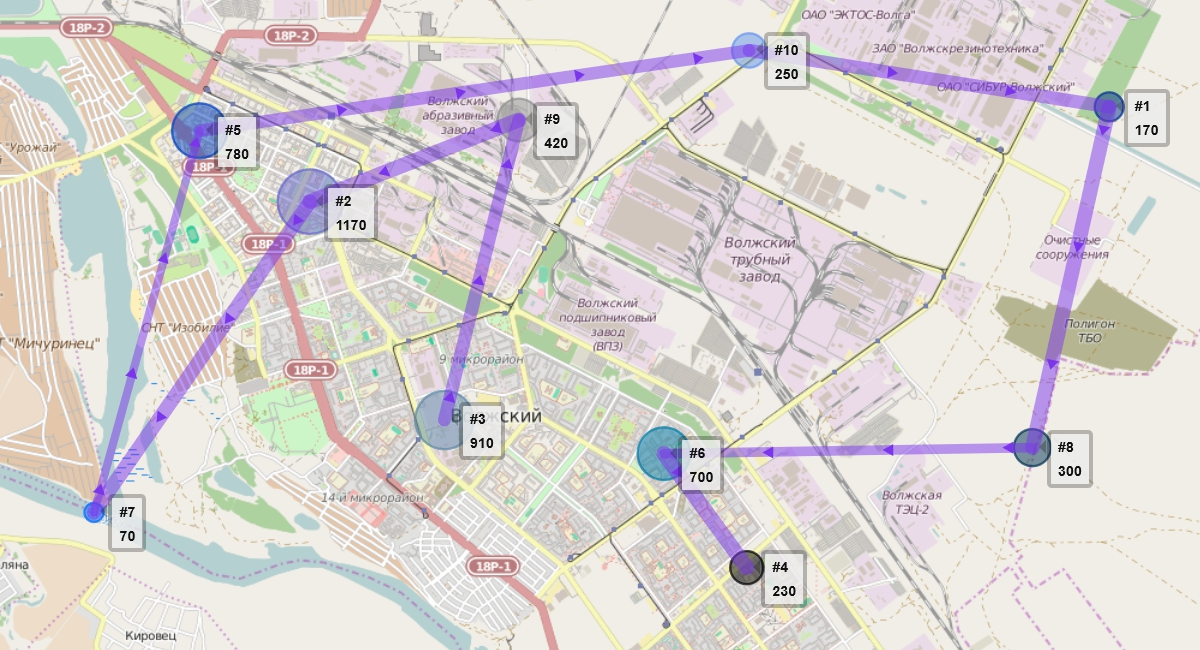
\includegraphics[width=\textwidth]{simulated-annealing-03}
    \caption{Полученый список обхода: \( 3, 9, 2, 7, 5, 10, 1, 8, 6, 4 \)\\
        Значение целевой функции: \( 0.0971 \)}
    \label{fig:sim-ann-01}
    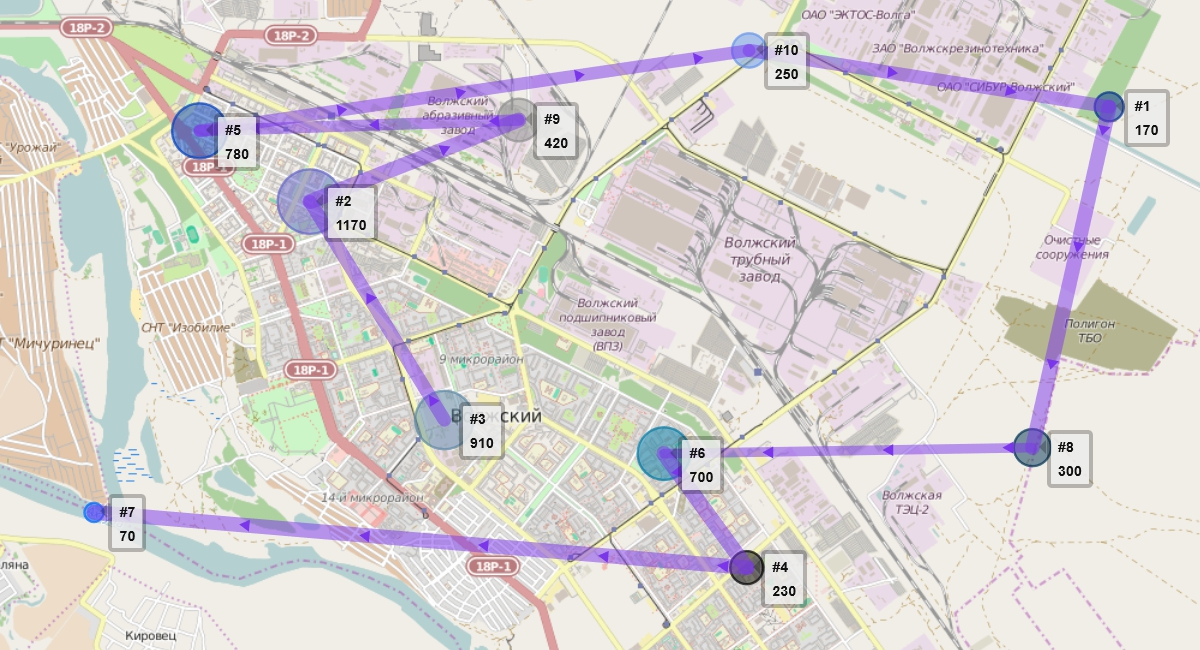
\includegraphics[width=\textwidth]{simulated-annealing-04}
    \caption{Полученый список обхода: \( 3, 2, 9, 5, 10, 1, 8, 6, 4, 7 \)\\
        Значение целевой функции: \( 0.0983 \)}
    \label{fig:sim-ann-02}
\end{figure}
\begin{figure}[ht!]
    \centering
    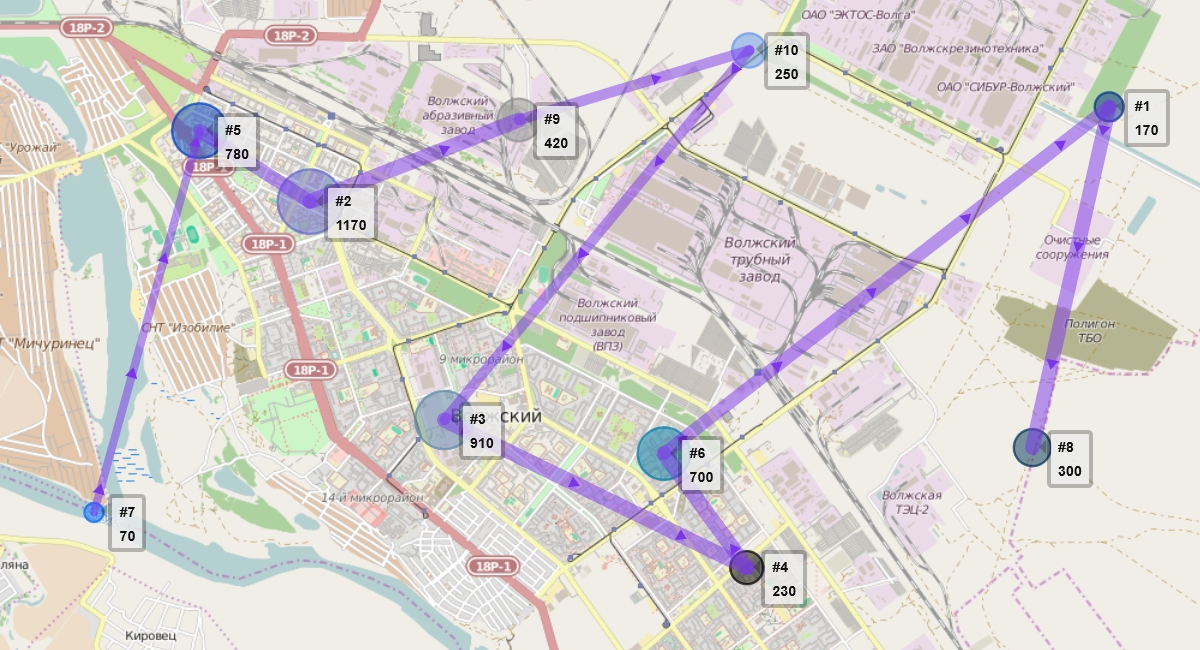
\includegraphics[width=\textwidth]{simulated-annealing-02}
    \caption{Полученый список обхода: \( 7, 5, 2, 9, 10, 3, 4, 6, 1, 8 \)\\
        Значение целевой функции: \( 0.1056 \)}
    \label{fig:sim-ann-03}
    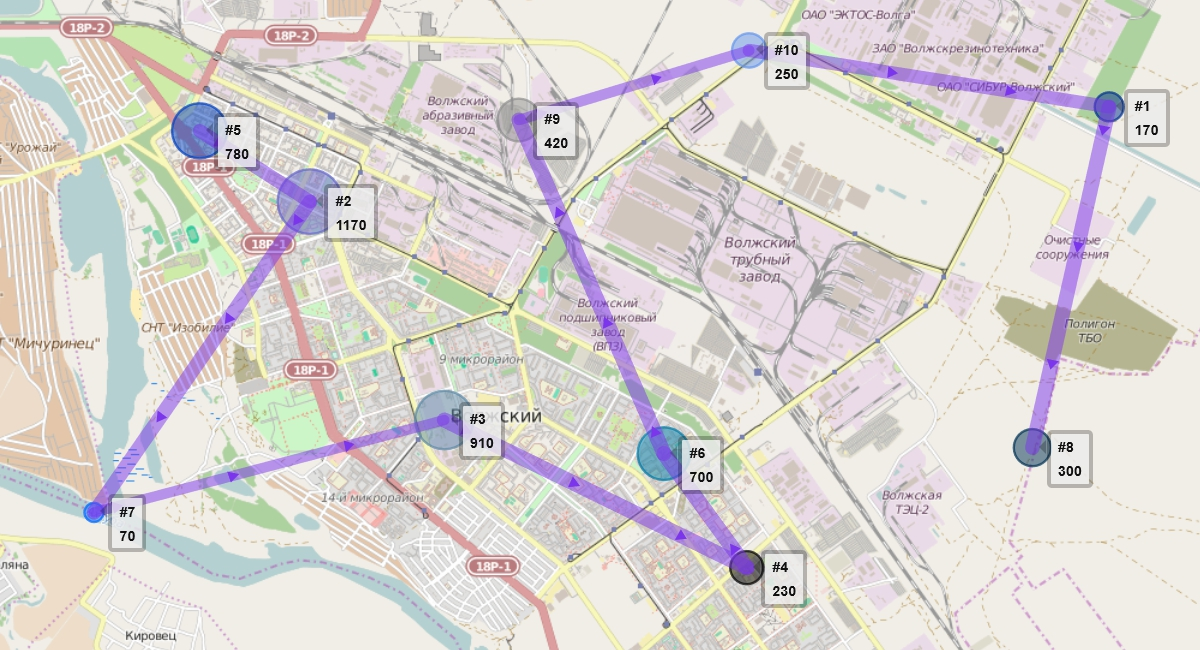
\includegraphics[width=\textwidth]{simulated-annealing-01}
    \caption{Полученый список обхода: \( 5, 2, 7, 3, 4, 6, 9, 10, 1, 8 \)\\
        Значение целевой функции: \( 0.1248 \)}
    \label{fig:sim-ann-04}
\end{figure}
\newpage

\subsection{Поиск с запретами}
Как и алгоритм имитации отжига, поиск с запретами является метаэвристикой, основанной на локальном поиске, 
где на каждой итерации выбирается лучшее решение в окрестности текущего решения в качестве нового текущего 
решения, даже если это приводит к увеличению стоимости решения.

Краткий анализ алгоритма:
\begin{itemize}
    \item лёгкая адаптация к сложным моделям;
    \item простота и возможность гибридизации с другими методами;
    \item возможность перехода между локальными оптимумами;
    \begin{itemize}
        \item использование списка запретов;
        \item хранение только \( l \) элементов списка;
    \end{itemize}
    \item выбор мер схожести для сравнения решений;
    \item вероятность \emph{застрять} в локальной окрестности;
\end{itemize}

\begin{algorithm}[ht!]
    \caption{Общий алгоритм поиска с запретами}
    \KwData{\( T \) -- длина списка запретов, \( N \) -- количество модификаций,\\
        \( A \) -- начальное решение}
    \KwResult{\( B \) -- результат алгоритма}
    \( l \leftarrow \) требуемая длина списка запретов \( T \)\;
    \( n \leftarrow \) количество модификаций \( N \)\;
    \( S \leftarrow \) начальное решение \( A \)\;
    \( B \leftarrow S \)\;
    \( L \leftarrow { S } \) список запретов длины \( l \) с записанным \( S \)\;
    \Repeat{достигнут предел по количеству итераций}{
        \If{Length(L) > l}{
            Удалить самый старый элемент из \( L \)\;
        }
        Выбрать решение \( R \) из \( S \)\;
        \For{n-1}{
            Выбрать решение \( W \) из \( S \)\;
            \If{\( W \notin L \) и \( (f(W) > f(R) \) или \( R \in L) \)}{
                \( R \leftarrow W \)\;
            }
            \If{\( R \notin L \) и \( f(R) > f(S) \)}{
                \( S \leftarrow R \)\;
                Записать \( R \) в \( L \)\;
            }
        }
        \If{\( f(S) > f(B) \)}{
            \( B \leftarrow S \)\;
        }
    }
    \label{alg:tabu-search}
\end{algorithm}

\emph{Основная проблема:} необходимо введение параметра отвечающий за число итерация, для предотвращения 
зацикливаний алгоритма.

\subsection{Семейство генетических алгоритмов}
Генетический алгоритм -- это эвристический алгоритм поиска, используемый для решения задач оптимизации и 
моделирования путём случайного подбора, комбинирования и вариации искомых параметров с использованием 
механизмов, аналогичных естественному отбору в природе. Является разновидностью эволюционных вычислений, 
с помощью которых решаются оптимизационные задачи с использованием методов естественной эволюции, таких 
как наследование, мутации, отбор и кроссинговер. Отличительной особенностью генетического алгоритма 
является акцент на использование оператора <<скрещивания>>, который производит операцию рекомбинации 
решений-кандидатов, роль которой аналогична роли скрещивания в живой природе.

Краткий анализ алгоритма:
\begin{itemize}
    \item кодирование информации в виде хромосом;
    \item использование операций скрещивания, селекции и мутации;
    \item реализация операций в задаче коммивояжера.
\end{itemize}

\begin{algorithm}[ht!]
    \caption{Общий вид генетического алгоритма}
    1. \emph{Инициализация}: порождение начальной популяции\;
    2. \emph{Выбор окрестности}: выбор операторов \emph{crossover} и \emph{mutation}\;
    3. \emph{Выбор родителя}: использование оператора селекции к текущей популяции\;
    4. \emph{Реализация шага}: использование операторов \emph{crossover}, 
        \emph{mutation}, \emph{hill climbing}, выбора потомка и родителя для получения 
        новой популяции\;
    5. Если критерии остановки не выполняются перейти к шагу 3 (продолжить эволюцию) 
        или перейти к шагу 1-3 (изменить критерии эволюции)\;
    \label{alg:genetic}
\end{algorithm}

\emph{Основная проблема:} представление графа сети в виде хромосом.

\clearpage

\subsection{Жадный алгоритм}
\label{sec:greedy-alg}
\subsubsection{Общее описание}
Поглощающий алгоритм (<<жадный алгоритм>>) -- тип алгоритмов оптимизации, которые на каждом шаге выбирают 
локально оптимальную альтернативу -- ту, которая приносит на этом шаге максимальную выгоду. Работают быстро, 
но обычно дают глобально неоптимальное решение, так как пропускают случай, когда лучше на данном шаге 
выбрать не самую лучшую альтернативу, но затем на следующем шаге получить значительный выигрыш.

Входные данные: полносвязный граф, в котором вершины заданы географическими координатами и количеством 
точек отправления или назначения в кластере, а рёбрам предписаны веса, которые означают потребность в 
перевозке пассажиров между кластерами. Это может быть, например, количество необходимых перевозок в час в то 
или иное время суток (например, в часы пик или же наоборот в спокойное время).

В результате кластеризации исходных данных на предыдущем этапе получен полносвязный граф, вершины 
которого -- центры кластеров (заданы географическими координатами и количеством точек отправления или 
назначения в кластере). Веса рёбер -- потребность в перевозке пассажиров между кластерами. 

\subsubsection{Схематическое представление}
Последовательность работы алгоритма описывается следующими шагами:
\begin{enumerate}
    \item определяем ребро графа с максимальной потребностью в транспорте;
    \item выбираем из двух вершин, которые это ребро соединяет, одну, с максимальным количеством 
        пассажиров в ней;
    \item делаем первый шаг из этой вершины в другую, выбирая то ребро, которое имеет максимальную 
        потребность;
    \item из этой вершины делаем шаг в следующую, тоже выбирая ребро с максимальной потребностью:
    \begin{enumerate}
        \item если два ребра имеют одинаковую пропускную способность, то выбираем любое;
        \item если ребро имеется в списке, то выбираем следующее по пропускной способности;
    \end{enumerate}
    \item строим до тех пор, пока длина маршрута не превысит пороговое значение;
    \item переходим к пункту 1, выбрав следующее по пропускной способности ребро.
\end{enumerate}

\subsubsection{Результат работы}
Пример работы алгоритма приведен на рисунке \ref{img:greedy-01}.
\begin{enumerate}
    \item Выбираем ребро с потребностью перевозки 300.
    \item Выбираем кластер с количеством точек 500.
    \item Первый шаг: начинаем маршрут с ребра 300.
    \item Второй шаг: выбираем ребро 200.
    \item Третий шаг: выбираем ребро 100.
\end{enumerate}

\begin{figure}[h!]
    \centering
    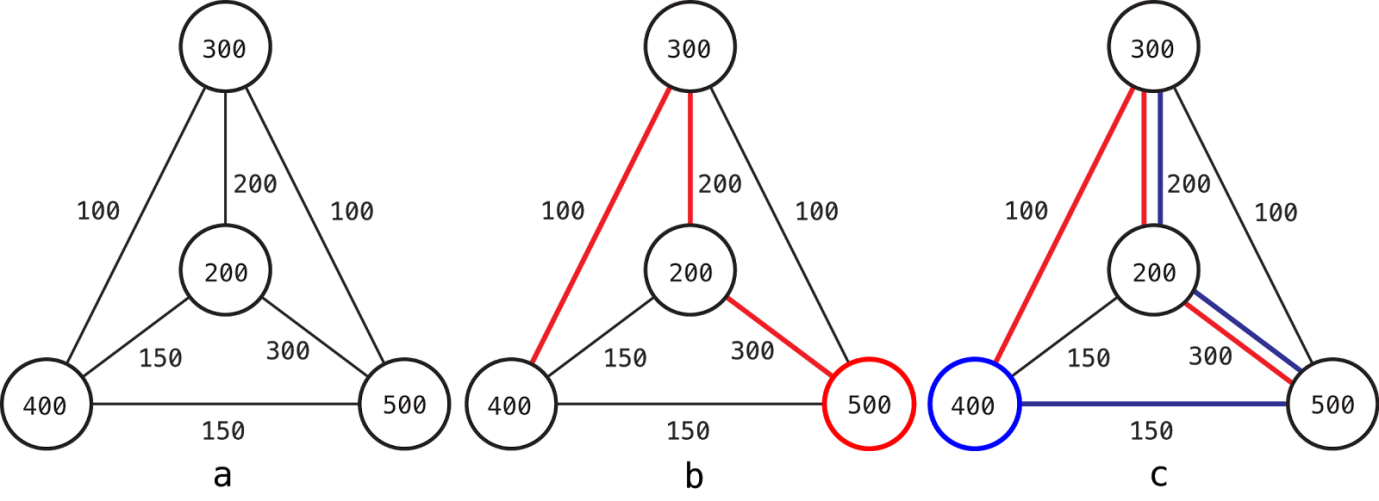
\includegraphics[width=0.8\textwidth]{greedy-01}
    \caption{Пример реализации алгоритма\\
        a -- исходный граф;\\
        b -- первый построенный маршрут (вершина начала пути выделена красным);\\
        c -- второй построенный маршрут (вершина начала пути выделена синим).
    }
   \label{img:greedy-01}
\end{figure}

\section{Алгоритм минимального увеличения длины}
\label{sec:second_alg}
\subsection{Общее описание}
Формирование начальной сети маршрутов, используя принцип <<минимального>> увеличения длины маршрута при 
включении нового пункта. Идея алгоритма заключается в итеративном добавлении в существующие маршруты узлы, 
минимально увеличивающие длину исходных маршрутов. 

На вход алгоритма подаются: \( N_r \) -- число маршрутов в сети, \( N_c \) –- число узлов 
(центров кластеров), \( C_t \) – множество терминальных узлов (определенных посредством построения 
окружности, содержащей все узлы), \( C_{nt} \) -- множество нетерминальных узлов (сумма элементов множества 
терминальных и нетерминальных узлов равна числу центров кластера), матрица длин размером 
\( ||{C_{nt}} + {C_{t}}|| \times ||{C_{nt}} + {C_{t}}|| \). Заметим, что \( C_t + C_{nt} = n_c \)

Выходом алгоритма является транспортная сеть \( RN \), содержащие непересекающиеся множество узлов, 
\( r_{i} = [p_{1}^{(i)}, \dots, p_{k}^{(i)}] \), где \( i = 1, \dots, n_r \). 

\subsubsection{Идея метода}
Данный алгоритм содержит следующие шаги
\begin{enumerate}
    \item[Шаг 1] Создать \( n_r \) прямых маршрутов, содержащих пары противоположных терминальных 
        узлов из \( C_t \) и добавить их в \( R_i \)
    \item[Шаг 2] Для каждого \( i \)-го маршрута из сети \( R_i \) выполнить:
    \begin{enumerate}
        \item[2.1] Выбрать \( i \)-тый маршрут из \( R_i \) и разделить его на пары и добавить их в \( PN \);
        \item[2.2] Найти такой узел \( C_t \), который минимально увеличивает длину маршрута из \( PN \) и 
            добавить новый маршрут, включающий данный узел, в \( RC \);
        \item[2.3] Составить \( ||RC|| \) вариантов новых маршрутов: один взятый из сети \( RC \), другой 
            из сети \( PN^{(R_{i})} \) и составить список кандидатов на замену в \( RCC \);
        \item[2.4] Оценить длины маршрутов в \( RCC \) и выбрать маршрут \( R^{\star}_{i} \) 
            с минимальной длиной;
        \item[2.5] Заменить \( R_{i} \) на $R^{\star}_{i}$ в маршрутной сети \( RN \);
        \item[2.6] Удалить узел \( c_{j} \) из \( C_{nt} \) добавленный в \( R^{\star}_{i} \). 
    \end{enumerate}
    \item[Шаг 3] Если \( C_t \) не пустое, перейти на шаг 2, иначе закончить построение.
\end{enumerate}

\subsection{Схематическое представление}
Псевдокод алгоритма представлен следующей схемой \ref{alg:min-length}.
\begin{algorithm}[ht!]
    \caption{Алгоритм построения маршрутной сети}
    \KwData{\( N_r, C_t, C_nt \)}
    \KwResult{\( RN \)}
    \For{\( i=1 \ldots N_r \)}{
        1. Построить \( R_{i} \) прямой маршрут включающий пару терминальных кластеров из \( C_t \)\;
        2. Добавить \( R_{i} \) в \( RN \);\
    }
    \While{\( C_{nt} \) не пусто}{
        \For{\( i=1 \ldots N_r \)}{
            1. Выбрать \( R_{i} \) из \( RN \), \( R_{i} = [n_1, n_2, \ldots n_{R}] \)\;
            2. Разделить \( R_{i} \) на пары
                \( PN^{(R_{i})} = [[n_1, n_2] , [n_2, n_3], \ldots, [n_{R-1}, n_{R}]] \)\;
            3. Инициализировать список \( RC \)\;
            4. \For{пары \( [n_x, n_y] \) из \( PN^{(R_{i})} \)}{
                4.1 Найти узел минимально увеличивающий маршрут \( [n_x, n_y] \), т.е. найти узел \( c_j \)
                    из \( C_{nt} \), где \( j = argmin (|len(n_x, n_y)  - (len(n_x, c_j, n_y))|) \)\;
                4.2 Добавить \( [n_x, c_j, n_y] \) в \( RC \)\;
            }
            5. Составить \( ||RC|| \) вариантов новых маршрутов: один взятый из сети \( RC \), другой 
                из сети \( PN^{(R_{i})} \) и составить список кандидатов на замену в \( RCC \)\;
            6. Посчитать длины маршрутов в \( RCC \) и выбрать маршрут \( R^{\star}_{i} \) с 
                минимальной длиной\;
            7. Заменить \( R_{i} \) на \( R^{\star}_{i} \) в \( {RN} \)\;
            8. Удалить узел \( c_{j} \) входящий в \( R^{\star}_{i} \) из \( C_{nt} \)\;
        }
    }
    \label{alg:min-length}
\end{algorithm}

\subsection{Объяснение работы}
Поясним работу данного алгоритма на простом примере. Имеем некоторый набор терминальных кластеров 
\( A, A', B, B' \) (\( C_t \)) и нетерминальных \( C, D, \) \( E, F \) (\( C_{nt} \)). Количество маршрутов для 
построения \( n_r = 2 \). Необходимо построить два маршрута на основе входных данных.

Первым шагом является определение прямых маршрутов, которые включают только терминальные узлы. Условимся, 
что для первоначального маршрута и используются противоположные узлы, т.е. расположенные напротив друг друга. 
В данном случае получаем список содержащий два узла \( R_i = [AA', BB'] \). Рисунок \ref{fig:route_first} 
иллюстрирует данное начальное распределение маршрутов.

\begin{figure}[ht!]
    \centering
    \begin{subfigure}{0.3\textwidth}
        \centering
        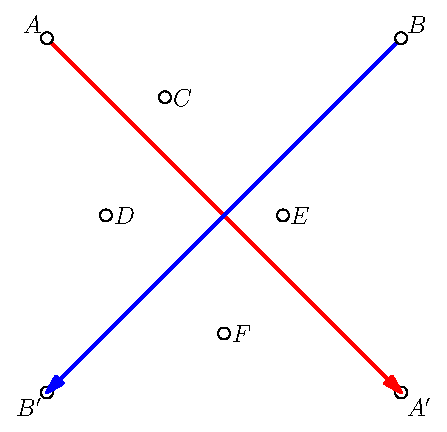
\includegraphics[width=\textwidth]{route01}
        \caption{Первоначальная маршрутная сеть включающая \( n_r \) прямых маршрутов с терминальными узлами.}
        \label{fig:route_first}
    \end{subfigure}
    \begin{subfigure}{0.3\textwidth}
        \centering
        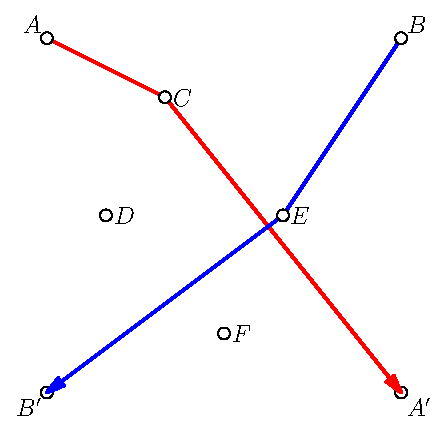
\includegraphics[width=\textwidth]{route02}
        \caption{Маршрутная сеть после первой итерации алгоритма.}
        \label{fig:route_second}
    \end{subfigure}
    \begin{subfigure}{0.3\textwidth}
        \centering
        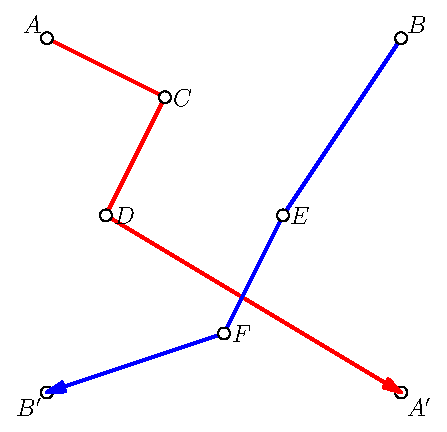
\includegraphics[width=\textwidth]{route03}
        \caption{Окончательная версия маршрутной сети.}
        \label{fig:route_third}
    \end{subfigure}
    \caption{Схематичное представление работы алгоритма}
    \label{fig:route}
\end{figure}

Далее, выбираем из первый элемент из списка \( R_i \) и разбиваем его на пары. На данном шаге, так как 
в маршруте только два узла, имеем только одну пару \( PN = [AA'] \).

Далее, конструируем набор маршрутов добавлением нового элемента в середину пары в существующие маршруты 
из \( PN \). В данном случае имеем следующий набор \( ACA', ADA', AEA', AFA' \).

Для полученных четырёх маршрутов рассчитаем длину для каждого и выбираем с наименьшим значением 
(в нашем случае это \( ACA' \)). Добавляем \( ACA' \) в список маршрутов \( RC = [ACA'] \).

Далее, составляем все варианты новых маршрутов из \( RC \) и \( PN \). В данном случае получаем только 
один \( ACA' \) и добавляем его в список \( R^{\star}_{i} \). Узел \( С \) удаляем из списка \( C_nt \).
Проделываем аналогичные действия и для второго маршрута -- получаем новый маршрут \( BEB’ \).
Рисунок \ref{fig:route_second} отражает маршрутную сеть после первой итерации алгоритма.

На второй итерации цикла имеем список маршрутов \( R_i = [ACA', BEB'] \). Используя \( ACA' \) можно 
сконструировать две пары \( PN=[AC, CA'] \).

Последовательно добавляя каждый нетерминальный кластер имеем следующий список \( ADC, AFC, CDA', CFA' \). 
Допустим, что минимальным из них является \( CDA' \).

Составляем различные варианты из \( CDA' \) и \( AC \), \( CA' \) получаем новый \( ACDA' \). Добавляем 
полученный маршрут в \( R^{\star}_i \) и удаляем узел \( D \) из \( C_nt \).

Аналогично для второго маршрута из \( R_i \) получаем \( BEFB' \).

Так как \( C_nt \) не содержит больше узлов (пустой список), то алгоритм заканчивает свою работу.

Рисунок \ref{fig:route_third} отражает окончательный этап алгоритма.

\subsection{Использование алгоритма выпуклой оболочки}
Для поиска терминальных кластеров, для начальной сети прямых маршрутов (шаг 1), используется простая идея 
основанная на идее алгоритма выпуклой оболочки.

Для всех заданных узлов создаётся выпуклая оболочка. Это помогает нарисовать круг описанный вокруг данной
оболочки. Так как у нас есть ряд маршрутов в качестве входного параметра, то определяем \( 2\cdot N_r \) 
равномерно расположенных узлов на построенной окружности. Узлы расположенные напротив друг друга являются 
квази-узлами отправления/назначения для маршрутной сети. Для определения реального узла отправления/назначения 
выбираем вокруг квази-узла некоторый \( \epsilon \) радиус и находим все принадлежащее узлы к данной окрестности.
Так как список может попасть больше чем один узел, то необходимо произвести сортировку данных узлов по 
количеству людей находящимся в нём и выбирать с наибольшим количеством.

\subsection{Результаты работы}
Алгоритм был апробирован на различных тестовых данных для различных значений числа маршрутов. 
Результат работы алгоритма представлен на \ref{img:min-length-01}.
\begin{figure}[h!]
    \centering
    \begin{subfigure}{0.75\textwidth}
        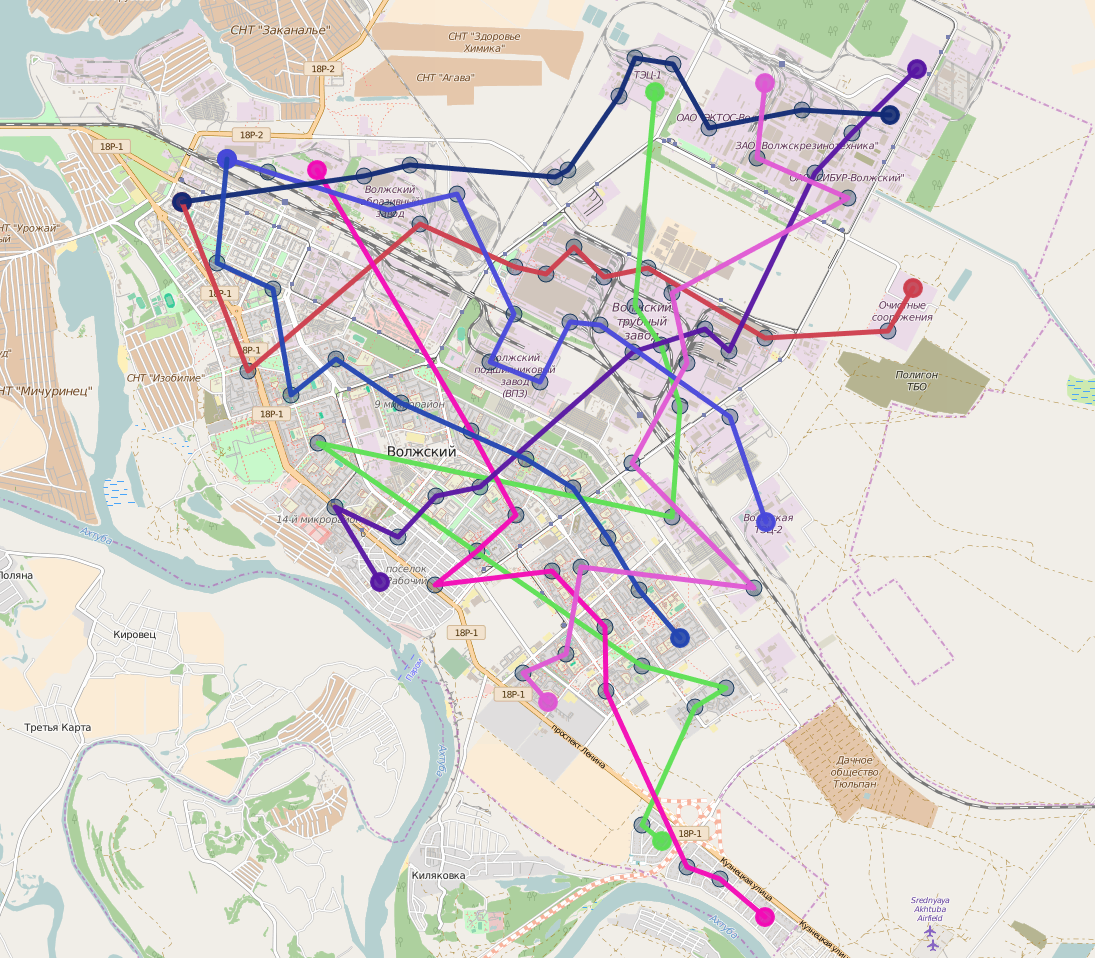
\includegraphics[width=\textwidth]{minimal-01}
        \caption{Построением маршрута по графу}
        \label{fig:graph}
    \end{subfigure}
    \begin{subfigure}{0.75\textwidth}
        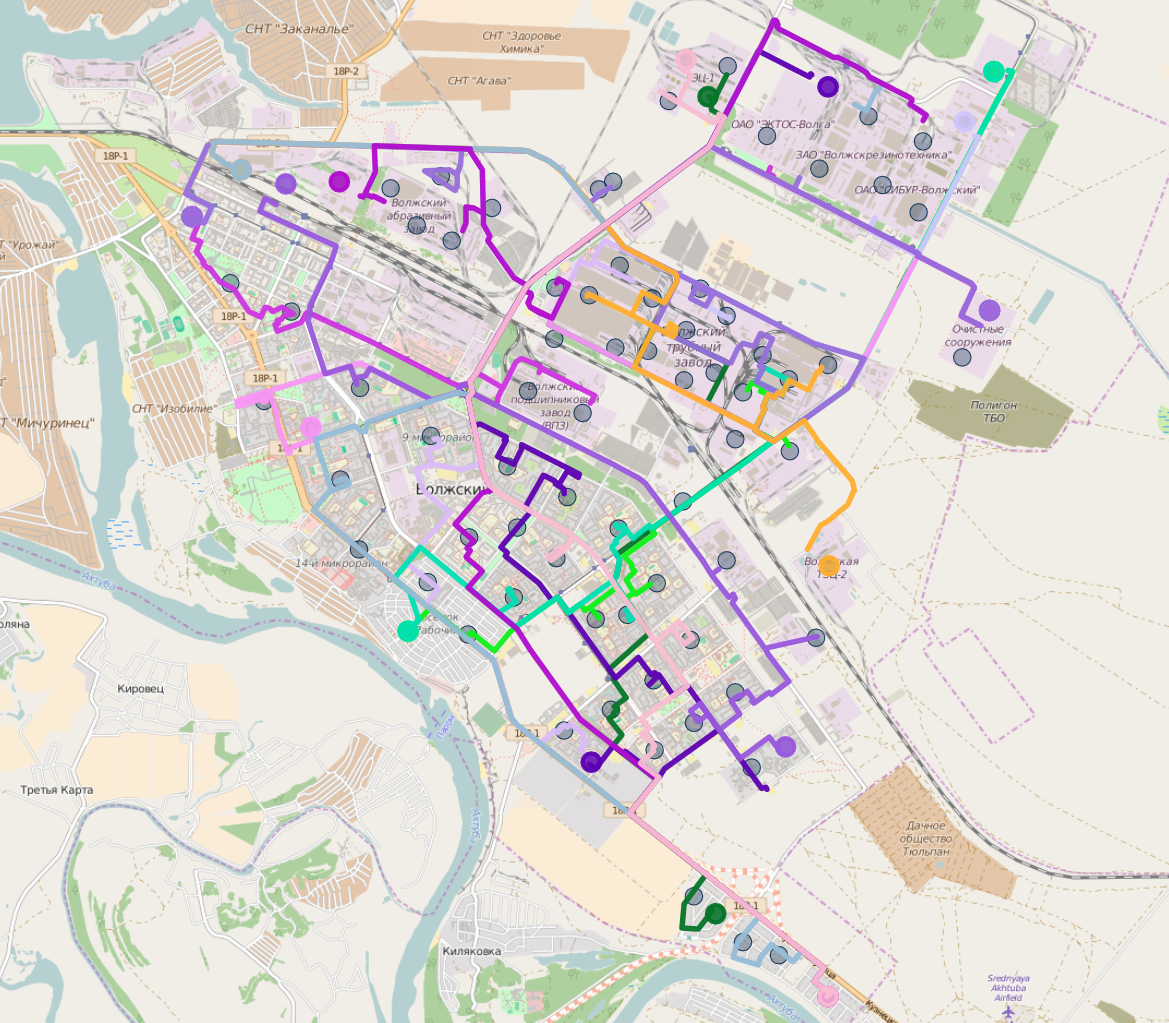
\includegraphics[width=\textwidth]{minimal-02}
        \caption{Построением маршрута по дорогам}
        \label{fig:osrm}
    \end{subfigure}
    \caption{Визуализация результата работы алгоритма формирования начальной сети маршрутов, 
        использующий принцип <<минимального>> увеличения длины маршрута при включении нового пункта%:\\
        % a -- с построением маршрута по графу\\
        % b -- с построением маршрута по дорогам
    }
   \label{img:min-length-01}
\end{figure}

\clearpage

\section{Алгоритм модификации начальной сети маршрутов}
\label{sec:third-alg}
% ---------------
% 3 метод -- WIP
% ---------------
\emph{Модификация начального варианта сети маршрутов общественного транспорта с целью минимизации функции 
затрат и генерация вариантов альтернатив сетей}
\subsection{Общее описание}
Модификация начального варианта сети маршрутов общественного транспорта осуществляется с использованием идеи 
итерационного эволюционного преобразования исходного маршрута. Предлагается эволюционный алгоритм, 
использующий операции мутации и кроссовера для оптимизации длины сети маршрутов [19].

\subsection{Идея метода}
Эволюционный алгоритм представлен следующей последовательностью шагов. 
\begin{enumerate}
    \item[1.] Если выбрана стратегия формирования единственного начального маршрута, то 
    \begin{enumerate}
        \item[1.1.] Сформировать единственный маршрут жадным алгоритмом.
        \item[1.2.] Разрезать маршрут на \( k \) маршрутов (где \( k \) -- изначально заданное число 
            маршрутов).
    \end{enumerate}
    \item[2.] Если выбрана стратегия формирования начальной сети, то перейти на шаг 3.
    \item[3.] Оценить качество сети маршрутов (с использованием критериев качества, например длины 
        маршрутной сети).
    \item[4.] Применить операцию кроссовера и мутации для получения новой генерации транспортной 
        сети \cite{bib:20}.
    \begin{enumerate}
        \item[4.1.] Оценить качество новой сети маршрутов.
        \item[4.2.] Если новая популяция лучше предыдущей, сохранить ее.
        \item[4.3.] Если новая популяция хуже предыдущей, отклонить. 
    \end{enumerate}
    \item[5.] Повторить, пока не выполняется условие останова.
\end{enumerate}

\subsection{Схематическое представление}
\subsection{Результаты работы}

\section{Заключение}